\documentclass{article}
\usepackage{tikz}
\usetikzlibrary{shapes.geometric}

\begin{document}

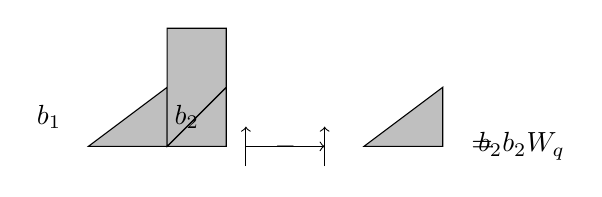
\begin{tikzpicture}[scale=0.5]
    % Define the dimensions
    \def\bOne{2}
    \def\bTwo{1.5}
    
    % Draw the first triangle
    \draw[fill=gray!50] (0,0) -- (\bOne,0) -- (\bOne,\bTwo) -- cycle;
    
    % Draw the second triangle
    \draw[fill=gray!50] (\bOne,0) -- (\bOne+\bTwo,\bTwo) -- (\bOne+\bTwo,0) -- cycle;
    
    % Draw the rectangle
    \draw[fill=gray!50] (\bOne,0) -- (\bOne+\bTwo,\bTwo) -- (\bOne+\bTwo,\bTwo+\bTwo) -- (\bOne,\bTwo+\bTwo) -- cycle;
    
    % Draw the labels
    \node at (-0.5*\bOne, 0.5*\bTwo) {$b_1$};
    \node at (0.5*\bOne+\bTwo, 0.5*\bTwo) {$b_2$};
    
    % Draw the minus sign
    \draw[->] (4,0) -- (6,0);
    \draw[->] (4,-0.5) -- (4,0.5);
    \draw[->] (6,-0.5) -- (6,0.5);
    \node at (5,0) {$-$};
    
    % Draw the second triangle again for subtraction
    \draw[fill=gray!50] (7,0) -- (9,0) -- (9,\bTwo) -- cycle;
    
    % Draw the equation
    \node at (10,0) {$=$};
    \node at (11,0) {$b_2 b_2 W_q$};
\end{tikzpicture}

\end{document}